\chapter{Neutrinoless Double-Beta Decay} \label{chap:theory} 
\section{The ``Little Neutral'' One}
The neutrino, the most elusive of all known fundamental particles, has a lot to say about ``life, the universe, and everything''~\cite{42}. In the 1920s, nuclear beta decay -- the process by which a neutron bound in a nucleus spontaneously decays into a proton by emitting an electron ($n\rightarrow p + e$) -- had thrown the field of physics into an uproar. The electron only carried a variable fraction of the surplus mass-energy of the decaying parent nucleus. This shocking revelation brought into question one of the most fundamental tenets of physics -- the law of conservation of energy. The theoretical physicist, Wolfgang Pauli, proposed that the missing energy was carried away by a yet undiscovered neutral and weakly-interacting particle, the neutrino: a ``desperate remedy'' he called it~\cite{pauli_letter}. Therefore, the beta-decay reaction actually results in a proton, electron, and an antineutrino ($\bar{\nu}$) -- the antimatter counterpart of the neutrino: $$n\rightarrow p + e + \bar{\nu}$$ ``I have done a terrible thing,'' Pauli lamented, ``I have postulated a particle that cannot be detected.''~\cite{pauli_quote} Eventually experimental physicists Frederick Reines and Clyde Cowan proved Pauli wrong nearly 30 years later~\cite{neutrino_discovery}. Thus, the age of experimental neutrino physics began, and physicists became experts at detecting vanishingly rare events with increasingly big detectors. 

\section{Ghosted by the Ghost Particle}
Double-Beta decay (\twovbb{}) is a second order electroweak process and, thus, much rarer than the well known single-beta decay. Single-beta decay is not energetically allowed in certain even-even nuclei; however, in such nuclei \twovbb{} can be observed. Two beta decays occur simultaneously, resulting in the emission of two electrons and two electron anti-neutrinos. It took 52 years from when Maria Goeppert-Mayer first postulated \twovbb{} in 1935~\cite{2vbb}, until it was first observed in $^{82}\text{Se}$~\cite{2vbb_obs}. Then again, the half-life of this isotope is over 9 orders of magnitude above the age of the universe.  This process has now been observed in various naturally existing isotopes with half-lives above $10^{18}$ years. In addition, a related process, double-electron capture, was recently observed by the XENON1T collaboration in $^{124}\text{Xe}$. This is the rarest decay ever observed, with a half-life of $1.8\times10^{22}$ years~\cite{ee_cap}.

The observation of even rarer decays is now within grasp with advances in low background measurement techniques. If neutrinos are Majorana particles, an even rarer event -- neutrinoless double-beta decay (\novbb{}) -- can occur. As opposed to \twovbb{}, no anti-neutrinos would be emitted, thus violating lepton number conservation~\cite{0vbb_theory}. Here, the two electrons carry away all the energy of the decay, producing a peak at the end of the broad \twovbb{} summed electron energy spectrum. This mono-energetic peak is the key experimental signature of \novbb{}. Via light Majorana neutrino exchange, the anti-neutrinos are exchanged as a virtual particle in the nucleus. More exotic mechanisms for \novbb{} have been proposed; nevertheless, regardless of the mechanism, the observation of such a phenomenon would imply that neutrinos are Majorana particles, and as such, they constitute their own anti-particles~\cite{valletheo}. From this point in the text forward, light Majorana neutrino exchange is assumed as the underlying process driving \novbb{}.

In 1937, Wendel Furry invoked Ettore Majorana's theory to propose \novbb{} as alternate mode for $\beta\beta$ decay. Since parity conservation was assumed, Furry postulated that \novbb{} would proceed at a much higher rate than \twovbb{}~\cite{wendell}. However, the opposite has been observed. Even though the leptonic phase space factor for \novbb{}, $G_{0\nu}$, is about 5 orders of magnitude greater than for \twovbb{}, its rate, $(T^{0\nu}_{1/2})^{-1}$, is greatly suppressed by a Majorana mass term, \mbb, such that
\begin{equation}
(T^{0\nu}_{1/2})^{-1} = G_{0\nu}(Q_{\beta\beta},Z)|M_{0\nu}|^2\left(\frac{\langle m_{\beta\beta} \rangle}{m_e}\right)^2~,
\label{eq:rate}
\end{equation}
where $Q_{\beta\beta}$ is the $Q$-value of the decay, $m_e$ is the electron mass, and $M_{0\nu}$ the dimensionless nuclear matrix element (NME) for the decay~\cite{Engel_2017}. The rate is the only observable; thus, $G_{0\nu}$ and the NME must be calculated to extract \mbb{}. If \novbb{} is observed, the knowledge of these factors would contribute to the determination of the underlying model for lepton number violation. Phase space factors depend on the $Q_{\beta\beta}$, the number of particles and the charge of the final state nucleus, $Z$, and have been recently re-calculated to greater precision~\cite{phasespace,phasespace2}. In contrast with the well known, $G_{0\nu}$, NME values for the same isotope differ in factors of 2 -- 3 from each other depending on the model used. When these models are applied to \twovbb{}, the predicted rates are always higher than those measured experimentally. Thus, the calculated NMEs are too large~\cite{jouniga}. The standard remedy is to introduce a quenching factor on the axial coupling constant, $g_A$, which differs for each NME and thus adds to the NME's uncertainty. However, more robust NME models can reduce quenching as shown in a recent publication~\cite{reduced_quenching}. 

Rapid progress in \textit{ab-initio} approaches will soon allow for a more precise computation of these matrix elements and set uncertainties for each one \cite{Engel_2017}. Although \textit{ab-initio} calculations were originally limited to very light nuclei, the NME for $^{48}$Ca has been very recently calculated in this framework~\cite{ca48}. In this respect, the relatively low atomic number of $^{48}$Ca and \geEn{} constitutes an advantage over other \novbb{} candidates. This poses an exciting scenario for the search for \novbb{}. As many tonne-scale experiments are entering their R\&D phase, improved calculations of matrix elements will inform these searches, and ultimately allow for the extraction of \mbb{} if \novbb{} is observed. The uncertainties in the current NMEs highlight the need for a multi-isotope \novbb{} experimental program to determine the effective Majorana mass. Additionally, if a peak is observed at \Qbb{} in one isotope there is the possibility that it could originate from an unknown background. However, if the \Qbb{} peak is observed across multiple isotopes, a strong claim can be made about the discovery of \novbb{}. 

Although neutrinos were long believed to be massless, neutrino oscillation experiments have shown that at least two of the neutrino mass eigenstates have non-zero mass~\cite{osc_sol,osc_atm}. The Pontecorvo-Maki-Nakagawa-Sakata (PMNS) matrix describes the mixing of neutrino mass eigenstates, as governed by three experimentally determined mixing angles. These angles have been observed to be large in comparison to their analogues in quark sector \cite{pdg_revparticlephys}. The superposition of mass states, dictated by the PMNS matrix, leads to the oscillation of neutrinos between different flavor states when these propagate through space. Neutrino oscillations in vacuum are only sensitive to the absolute value of the neutrino mass differences, $\Delta m^2_{ij} = m^2_i - m^2_j$, thus propagation through matter must be leveraged to determine not only the spacing between neutrino mass eigenstates but their ordering. This has been done for neutrinos that travel through the Sun, thus determining $\Delta m^2_{12}$. However, experiments are not yet sensitive enough to determine the sign of $\Delta m^2_{23}$ from neutrinos that are created in the atmosphere as products from cosmic rays, and only $|\Delta m^2_{23}|$ is known \cite{osc_rev}. Thus, the neutrino mass ordering remains partially ambiguous, leading to two possible scenarios, the so-called normal and inverted orderings (NO and IO respectively). Recent global fits of neutrino oscillation parameters moderately favor the NO over the IO at $2.7\sigma$, based on neutrino oscillation data~\cite{NH}. 

The effective Majorana mass, \mbb, depends on elements of the PMNS matrix, $U_{ej}$, and on the neutrino mass eigenstates, $m_j$, 
\begin{equation}
\langle m_{\beta\beta} \rangle = \left|U_{e1}^2 m_1 + U_{e2}^2 e^{i\alpha_{21}} m_2 + U_{e3}^2 e^{i\alpha_{31}} m_3 \right|~,
\label{eq:mbb}
\end{equation}
where $\alpha_{12}$ and $\alpha_{31}$ are two Majorana phases which are allowed if the neutrino is a Majorana particle~\cite{disc_prob0vbb}. Eq.~\ref{eq:mbb} can be rewritten in terms of the lightest neutrino mass $m_l$. The two possible mass orderings would therefore cause the two resulting expressions to diverge from each other if $m^2_l$ is of the order of $\Delta m^2_{ij}$, namely below $10^{-2}$ eV$^2$. The allowed values of \mbb~can be converted into a \Thalf~range via Eq.~\ref{eq:rate}. Applying the current limits given by direct mass measurements (sensitive to $m^2_{\nu_e} = \sum_{i}|U_{e1}|^2m^2_i$) and \novbb{} experiments, and the range of NMEs, gives \Thalf~ $ > 10^{26}$ years.  For the IO, \Thalf~cannot exceed $\sim 10^{28}$ years. The presence of the Majorana phases present a troubling scenario for the observation of \novbb{}. A careful tuning of these parameters in the NO expression would drive \mbb{}, and thus the \novbb{} rate, to zero. However, this scenario is unlikely as shown in a recent global fit which combines oscillation parameter data with limits from \novbb{} experiments and direct mass measurements (See Fig.~\ref{fig:globalfits}).
\begin{figure}[htb]
	\centering
	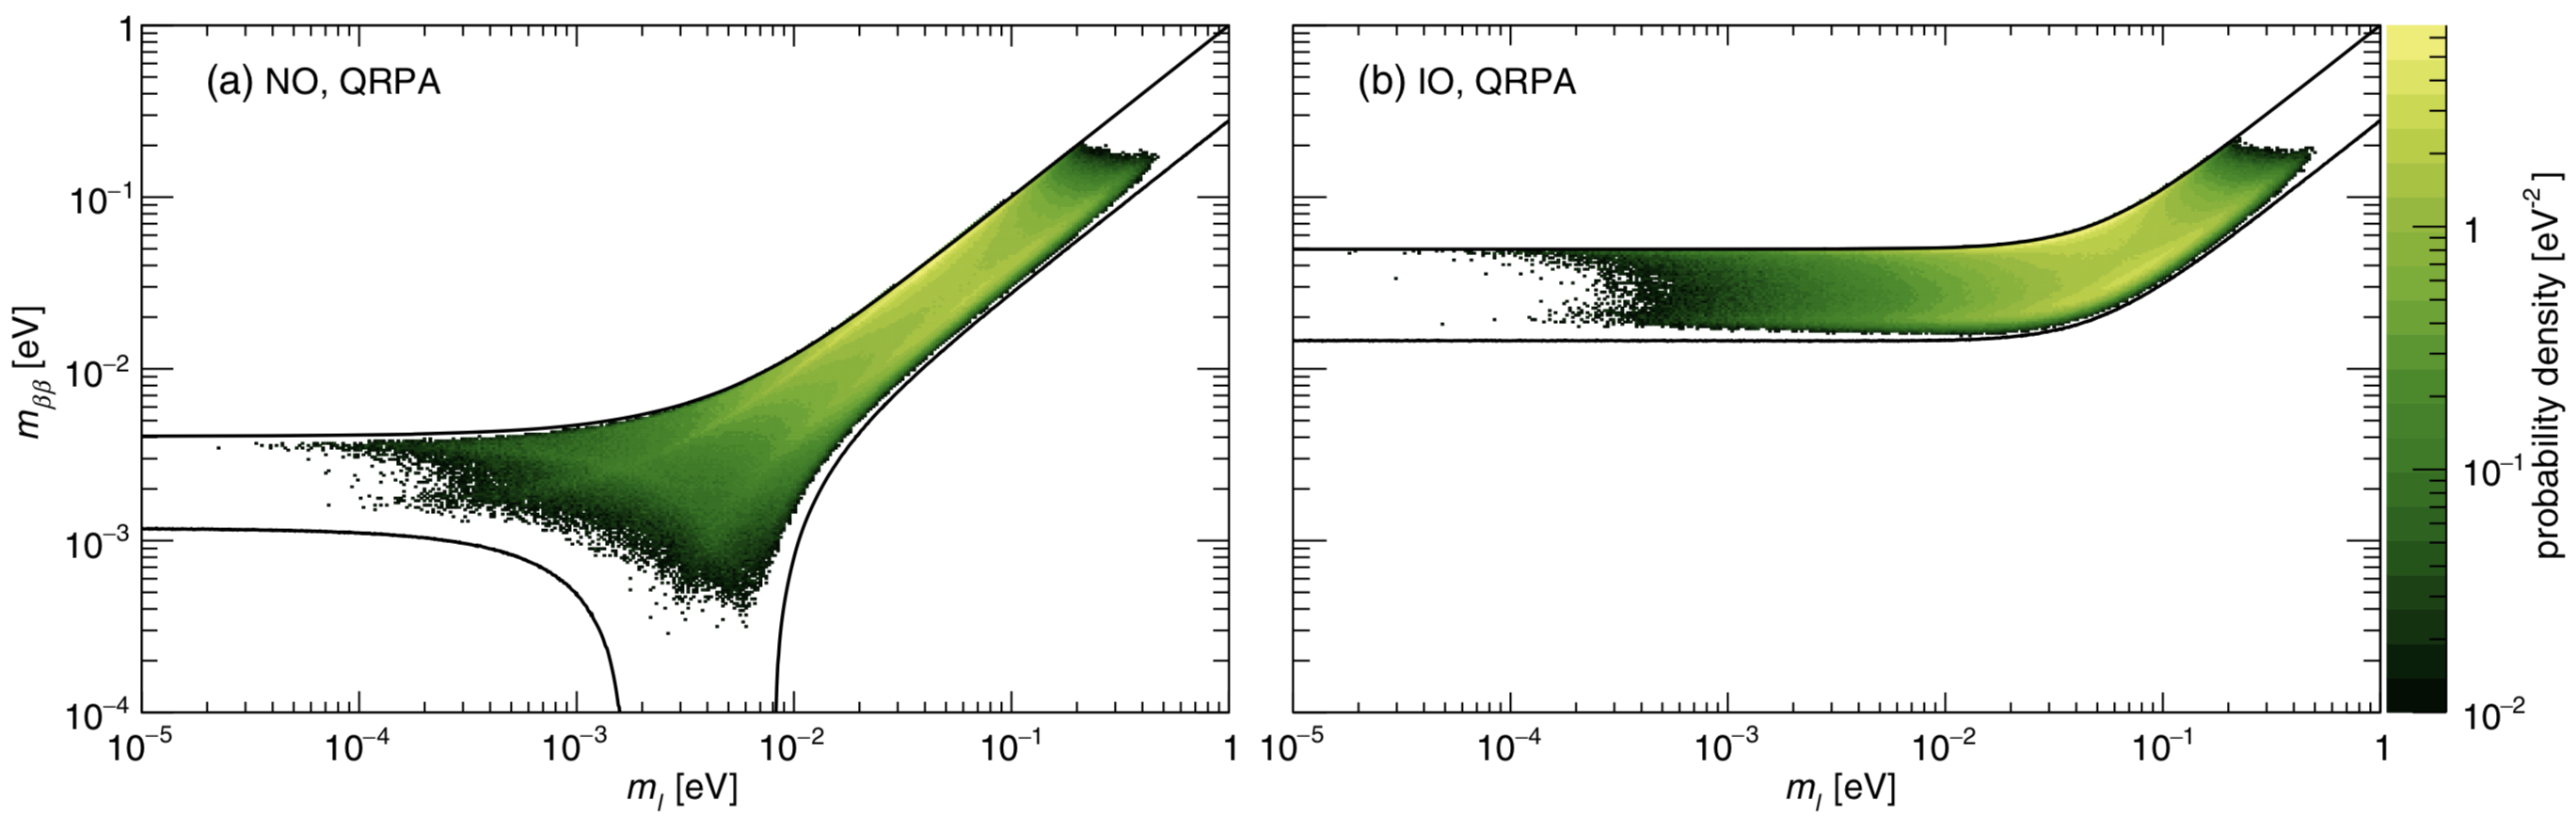
\includegraphics[width=1\linewidth]{figs/0vbb/globalfits}
	\caption{Marginalized posterior distributions for \mbb~and $m_l$ for the NO (a) and IO (b) assuming the absence of mechanisms that drive $m_l$ or \mbb~to zero~\cite{disc_prob0vbb}. The solid lines denote the region allowed by Eq.~\ref{eq:mbb} assuming 3$\sigma$ intervals of the neutrino oscillation parameters from Ref.~\cite{nufit}.}
	\label{fig:globalfits}
\end{figure}
This global fit predates the newest results from the KATRIN experiment, which cuts the previous limit on $m_{\nu_e}$ in half \cite{katrin, troitsk}. This new limit constrains the parameter space in Fig.~\ref{fig:globalfits} from the right, thus pushing \Thalf~down, slightly disfavoring the quasi-degenerate region. 

\section{Detecting Vanishingly Rare Events With Increasingly Big Detectors}

How does the \mbb{} parameter space inform the design of an experiment? Using Eq.~\ref{eq:rate} and assuming the neutrino is a Majorana particle with a \mbb{} that lies on the lower edge of the IO region, the corresponding half-life -- assuming the worst case NME -- is of the order of $10^{28}$ years. To design an experiment \textit{sensitive} to this half-life, half-life itself must be understood. In an ideal background free experiment, $N$ atoms are observed for a time $T$. In this experiment, all $D$ decays are detected. From radioactive decay theory $T_{1/2}$ is calculated as,
\begin{equation}
	T_{1/2} = \frac{\ln(2)}{k} 
\end{equation}
and the decay constant, $k$, can be determined from
\begin{equation}
	N - D = N\text{e}^{-kT}
\end{equation}
and approximated as $k = -\ln(1 - D/N)/T \approx D/(NT)$ when $D/N \ll 1$. Thus, for any rare decay search the half-life can be expressed as
\begin{equation}
	T_{1/2} = \ln(2)\frac{NT}{D} 
	\label{eq:Thalftheo}
\end{equation}

It maybe be that no decays are observed. This non-observation still provides valuable information. As will be seen, a limit on the half-life can be set. Eq.~\ref{eq:Thalftheo} requires some work when applied to a non-ideal experiment where background is present -- such as a \novbb{} search.  ``The sensitivity of an experiment to discover a signal is here defined as the value of \Thalf{} or \mbb{} for which the experiment has a 50\% chance to measure a signal with a significance of at least 3$\sigma$''~\cite{disc_prob0vbb}. This discovery sensitivity, $S^{0\nu(disc)}_{1/2}$, of an \novbb{} experiment is given by
\begin{equation}
	S^{0\nu(disc)}_{1/2} = \ln(2)\frac{N_{\beta\beta}T\epsilon_{tot}\epsilon_{res}}{S}~,
\label{eq:Thalfexp}
\end{equation}

where $T$ is the live time of the experiment, $N_{\beta\beta}$ is the number of \novbb{} candidate nuclei, and $\epsilon_{tot}$, $\epsilon_{res}$, correspond to the total and resolution efficiencies. Understanding the factors in Eq.~\ref{eq:Thalfexp} will allow the savvy experimenter to design an experiment sensitive to \novbb{} half--lives of the desired order. 

The efficiencies in Eq.~\ref{eq:Thalfexp} are included because not all signal events can be detected. Some signal events are discarded by the experimenter's analysis cuts. These are designed to maximize background rejection and minimize the sacrifice of signal events, $1 - \epsilon_{cut}$. Another signal-loss mechanism is of geometric origin. By constructing the detectors from the source material -- the \novbb{} isotope -- the vast majority of signal events are contained within the detector. However, the electrons produced in \novbb{} can escape or be absorbed in the dead layer of the detector. The containment efficiency ($\epsilon_{cont}$) -- the fraction of signal events that are contained in the active volume of the detector -- accounts for this. The total efficiency is given by: $\epsilon_{tot}=\epsilon_{cut}\epsilon_{cont}$.

$S$ now obtains a probabilistic nature as opposed to the previously known and idealized number of signal decays, $D$. $S$ denotes the number of signal events in the \novbb{} region of interest (ROI) for which a 50\% of experiments would report a fluctuation above background with a significance of at least 3$\sigma$. This statement requires some unpacking. Signal events will have an energy of \Qbb{}, however, the finite resolution of the experiment will force the experimenter to define a region of interest around this value to conduct the search.  Note that as the width of the ROI ($\Delta_{\text{ROI}}$) increases, the number of signal events contained in the region increases as well, this fraction is the aforementioned resolution efficiency. Assuming a Gaussian \novbb{} peak, the resolution efficiency takes the following form: $\epsilon_{res} = \text{erf}(\Delta_{\text{ROI}}/(2\sqrt2\sigma_E))$.  Here $\sigma_E$ is the energy resolution of the experiment. Therefore, $\epsilon_{res}$ will increase monotonically with the width of the ROI. However, a wider ROI will include more background counts and will thus increase $S$. Therefore, a savvy experimenter will maximize the figure of merit $\epsilon_{res}(\Delta_{\text{ROI}})/S(\Delta_{\text{ROI}})$ to set the ROI.

To calculate $S(\Delta_{\text{ROI}})$ the number of expected background counts in the ROI, $B$, must be known. A background estimation window (BEW) is used to derive this. In this energy window surrounding \Qbb{}, the background rate (also referred to as the background index), $\mu_b$, is calculated from the number of events in the BEW. These counts are normalized by the width of the BEW and the exposure of the experiment, $MT$, to produce a figure in units of c/(keV\,kg\,yr). The mass of the detector(s) is given by $M =  m_aN_{\beta\beta}/(\eta N_A)$, where $m_a$ is molar mass of the candidate isotope and $\eta$ the isotopic purity. The background rate, $\mu_b$, is assumed constant over the BEW to project $B = \mu_bMT\Delta_{\text{ROI}}$ background counts in the ROI.

$S$ is calculated as follows using the Poisson distribution, $p(n|\nu)$.
\begin{equation}
	\int_{0}^{C}p(n|B)dn = \alpha
	\label{eq:alpha}
\end{equation}
$\alpha$ corresponds the aforementioned significance level of 3$\sigma$ and is thus given by $\alpha = \text{erf}(3/\sqrt{2})$. Eq.~\ref{eq:alpha} uniquely determines the total number of counts in the ROI, C, which is used to solve for $S$ in Eq.~\ref{eq:beta}.
\begin{equation}
	\int_{0}^{C}p(n|B+S)dn = 1-\beta
	\label{eq:beta}
\end{equation}
$\beta = 0.5$ is set from the requirement that 50\% of experiments need to report a fluctuation above background. $S$ is calculated numerically, however, it is of interest to explore the following regimes. In the low background limit, $B<<1$, $S$ is constant, and thus $S^{0\nu(disc)}_{1/2}$ scales linearly with the exposure, $MT$. Note that $N_{\beta\beta}T$ can be replaced by $MT$ along with the appropriate constants in Eq.~\ref{eq:Thalfexp}. Conversely, with appreciable background, $S$ scales with the significance level times the square root of the number of background counts: $S \approx 3 \sqrt B = 3\sqrt{2n\sigma_E\mu_bMT}$. Thus, $S^{0\nu(disc)}_{1/2}$ scales as $\sqrt{MT}$. This finding highlights the importance of minimizing the background so that increases in exposure (which drive the cost of the experiment) can be fully effective. Strictly speaking, an experiment is not background free until $S$ is constant in relation to $B$. However, when there is a high chance of no counts occurring in the ROI, an experiment is considered to be quasi-background-free. 

To reach the required background levels and near unity detection efficiencies, the bulk of the detector must be made of the isotope in question. Many viable technologies exist, including noble gas time projection chambers (TPC), scintillating bolometers, and semiconductor diode detectors. A few general desirable properties of \novbb{} candidates are listed below, most of which can be deduced from Eq.~\ref{eq:rate} and Eq.~\ref{eq:Thalfexp}.
\begin{enumerate}[nolistsep]
	\item High natural abundance and isotope availability,  known enrichment process, and low cost maximizes the exposure, $MT$.
	\item Good energy resolution results in a narrow ROI, reducing backgrounds, and increasing $\epsilon_{res}$. 
	\item $Q_{\beta\beta}$ above the natural background $\gamma$ radiation threshold of 2615 keV. Any radiation above $Q_{\beta\beta}$ can result in energy depositions in the ROI by losing energy in matter interactions.
	\item High intrinsic radiopurity, lowers backgrounds. 
	\item Low \twovbb{} rate $(T^{2\nu}_{1/2})^{-1}$. Although high \twovbb{} rates in the ROI can be strongly suppressed with good energy resolution.
	\item Favorable NMEs and decay phase space factor.
	\item Low atomic number. The  isotope will be at the forefront of \textit{ab-initio} NME calculations.
	\item Well-developed detector technology.
	\item High density. The electrons are contained in smaller volumes and self-shielding is increased.
\end{enumerate} 

Monolithic TPCs can achieve high exposures and have some of the best limit setting capabilities in the field~\cite{exo200}. However, they suffer from modest energy resolution, degrading their discovery level sensitivity. As exemplified by Fig.~\ref{fig:sensitivity_comp}, in the low background regime, modest energy resolution will greatly suppress $S^{0\nu(disc)}_{1/2}$, while reducing the limit setting sensitivity to a lesser extent. In this respect, Ge detector based experiments have an advantage. Furthermore, they can be deployed in a phased approach, as opposed to TPCs, which once built cannot be made larger.

\geEn{} has long been at the forefront of the search for \novbb{}. The decay in question and Q-value are shown in Eq.~\ref{eq:ge76decay}.
\begin{equation}
	^{76}\text{Ge} \longrightarrow ^{76}\text{Se} + 2e^-,~Q_{\beta\beta} = 2039\text{\,keV}
	\label{eq:ge76decay}
\end{equation}
Ge detectors have long been a standard in the field of nuclear and particle physics and are very well posed for this search. The technology has set some of the best limits on \Thalf~to date~\cite{gerda,mjd_final}. As semiconductor diode detectors, their excellent energy resolution constitutes a major advantage. Additionally, the purification of Ge has been carried out further than any element on Earth~\cite{knoll}. Ge has a well-developed enrichment process, and can be readily enriched to 92\% \geEn{}. 

\section{A Hypothetical Tonne-Scale Experiment}\label{sec:design}

Now that all the factors of Eq.~\ref{eq:Thalfexp} are understood, a hypothetical experiment with discovery level sensitivity to a \novbb{} half-life of $10^{28}$ years can be designed. As a starting point, current low background technology is assumed. In particular, the {\MJDEMit}, a \geEn{}-based experiment, is used as a reference. The following performance parameters achieved by the {\DEMit} are used for the calculations below: $\mu_b = 6.6 \times 10^{-3}$\,c/(keV\,kg\,yr), FWHM$_E$ = 2.52\,keV, and $\Delta_\text{ROI}$ = 4.14\,keV~\cite{mjd_26,mjd_final}.

The exposure of the hypothetical experiment is chosen to be 10\,tonne\,yr, for example with 1\,tonne of pure \geEn{} detectors operating for 10 years. With this exposure, $B < 0.0027$ counts is required for the experiment to be truly background free (constant $S$). Nevertheless, applying the performance parameters listed above projects $B = 232$ background counts in the ROI. The value of $S$ for which 50\% of such hypothetical experiments would report a fluctuation above 3$\sigma$ is $S \approx 3\sqrt B =  46$. Plugging these values into Eq.~\ref{eq:Thalfexp} yields a discovery level sensitivity of $S^{0\nu(disc)}_{1/2} = 1.7 \times 10^{27}$ years. Therefore, even with the ultra-low background levels of the {\DEMit}, the $10^{28}$ level of sensitivity is not reached in the tonne-scale hypothetical experiment. The discovery level sensitivity varies with the energy resolution and the background rate as shown in Fig.~\ref{fig:sensitivity_disc}. In this parameter space, the yellow area represents the true background free level. Meanwhile, the hypothetical experiment lies in the lower right-hand edge of the plot. 
\begin{figure}[htb]
	\centering
	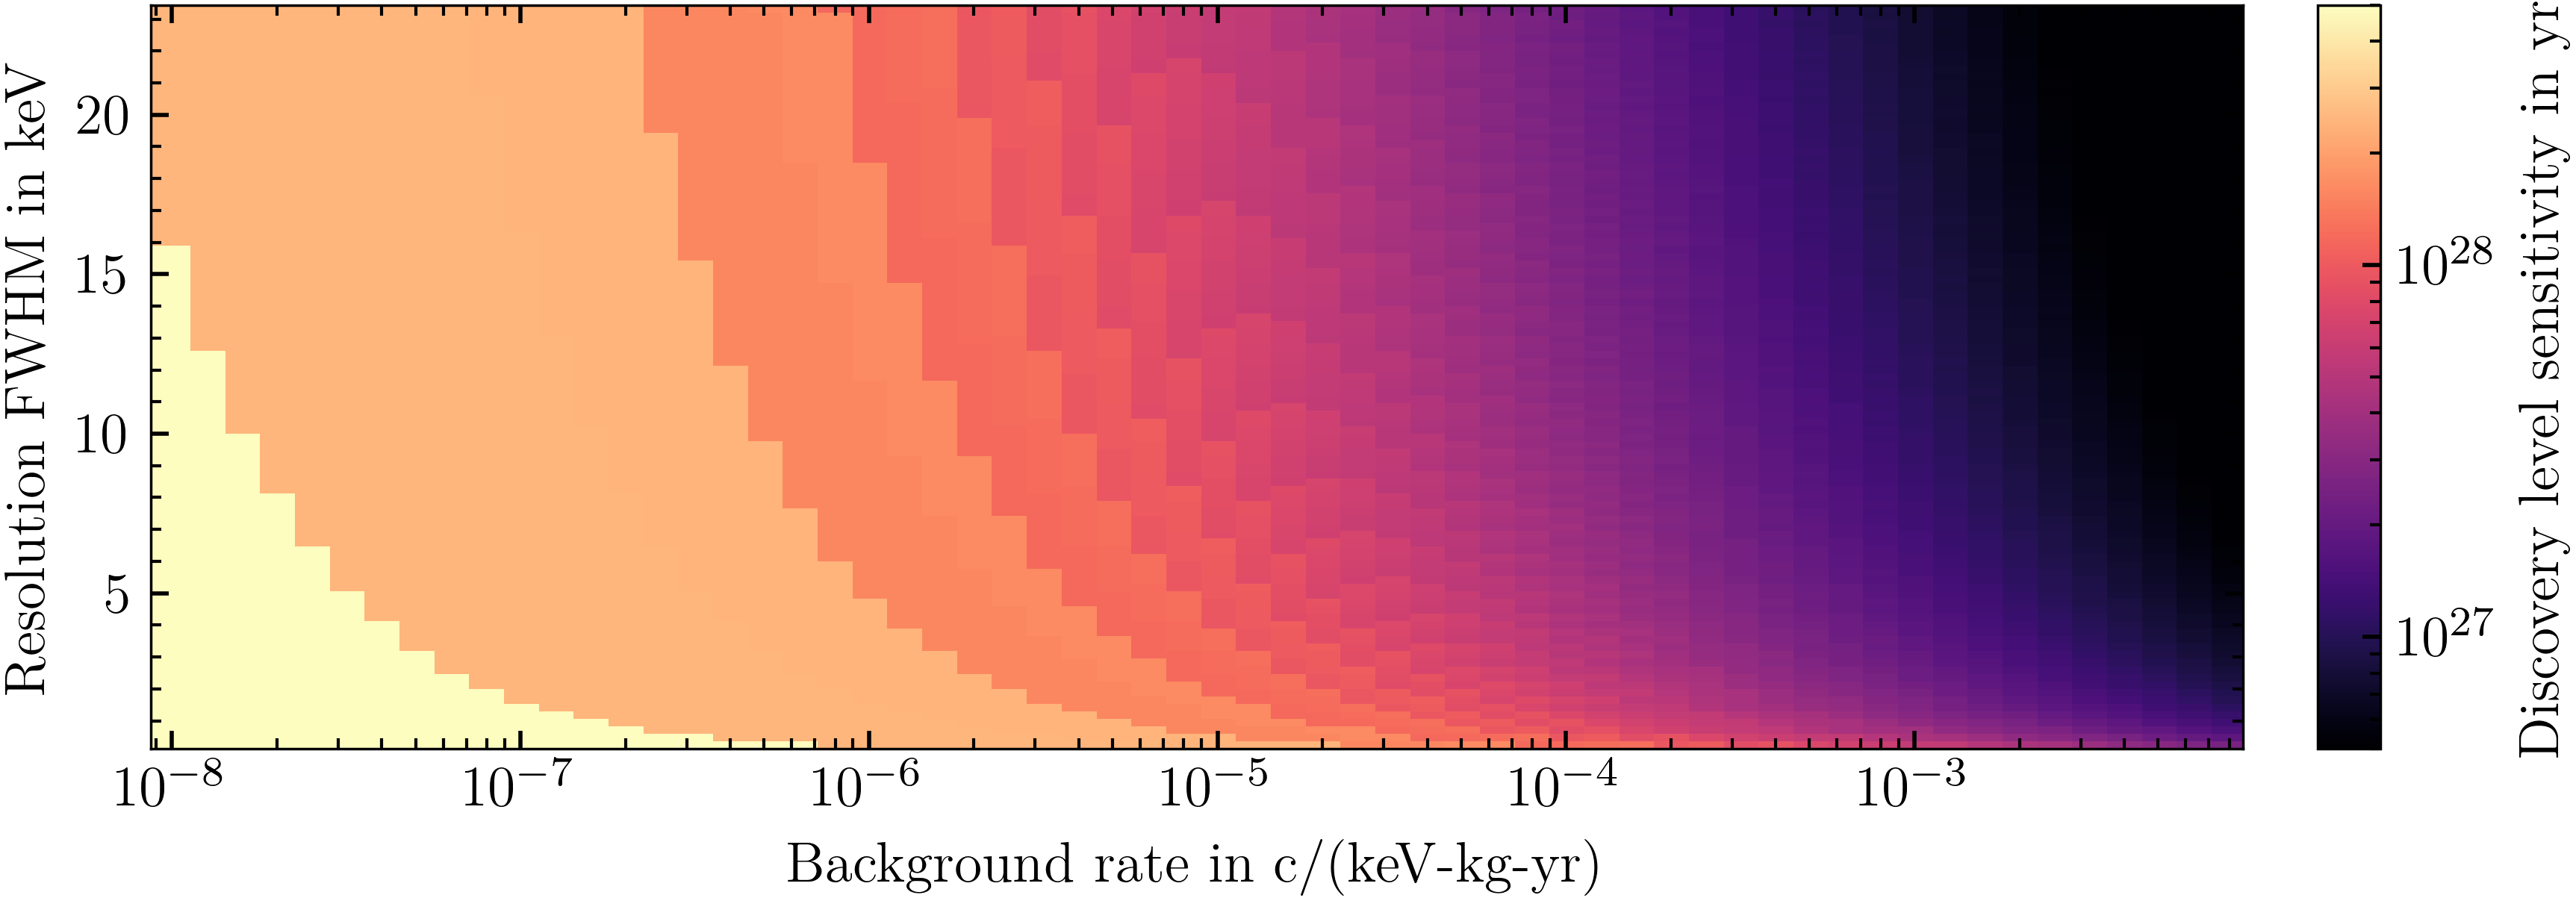
\includegraphics[width=6in]{figs/0vbb/discovery_sensitivity.png}
	\caption{Discovery level sensitivity, $S^{0\nu(disc)}_{1/2}$, for a 1 tonne \geEn{} experiment with 10 year live time, as it varies with respect to the background rate and and the energy resolution of the experiment. Assumes 100\% enrichment and $\epsilon_{tot} = 0.8$. In addition to the uniform background rate, contamination from the \twovbb{} is also considered. It is calculated as $B^{2\nu}= (T^{0\nu}_{1/2} S/T^{2\nu}_{1/2})( \sigma_E/Q_{\beta\beta})^6$ \cite{2vbb_background}. Note that this effect is almost negligible -- up to $\mathcal{O}(10^{-7})$ -- in this energy resolution range. ROI optimization is used. Background rate ranges from background free levels to that of the {\MJDEMit}. Energy resolution range is representative of many \novbb{} experiments. Code at \url{https://github.com/hervasa2/sensitivity.git}}
	\label{fig:sensitivity_disc}
\end{figure}

All, however, is not lost. The experiment can run longer or with increased the isotope mass. Unfortunately, this would produce diminishing returns as stated in the discussion of the behavior of $S$ and as seen in the right panel of Fig.~\ref{fig:legend_sensitivity}.  
\begin{figure}[htb]
	\centering
	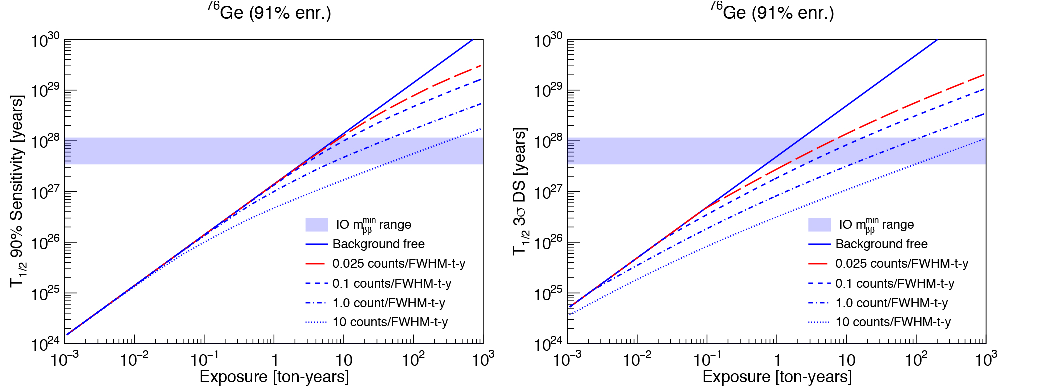
\includegraphics[width=6in]{figs/legend/legend_sensitivity.pdf}
	\caption{``The sensitivity to a \novbb{} decay signal in \geEn{} as a function of exposure and background for a (left) 90\% CL exclusion sensitivity and (right) 3$\sigma$ (99.7\% CL) discovery sensitivity (DS). Note, the background rates are normalized to a 2.5\,keV FWHM energy resolution.''~\cite{legend_pcdr}}
	\label{fig:legend_sensitivity}
\end{figure}
The hypothetical experiment has a background rate close to that of the dotted blue line in the figure. Nevertheless, a 700-fold reduction in background puts it on the same order as the dashed red line in the figure. This reduction of background rate to $\mu_b = 1 \times 10^{-5}$ c/(keV\,kg\,yr) (B = 0.3), yields $S = 4$, giving the desired $10^{28}$ discovery level sensitivity.

These are exactly the main design requirements for the next generation \novbb{} \geEn{} experiment, LEGEND-1000~\cite{legend}. That is, 10\,tonne\,yr of enriched exposure with a background rate  of $\mu_b < 1 \times 10^{-5}$ c/(keV\,kg\,yr). The drastic reduction in background levels might seem unattainable; however, a reduction factor of 10 has already been demonstrated by the GERDA collaboration~\cite{GERDA2020}. Additionally, in the hypothetical experiment, the effects of scaling up the {\MJDEMit}, were ignored: self-shielding and increased granularity help in background mitigation. For further details on these experiments, refer to Section~\ref{sec:experiments} and Chapter~\ref{chap:legend}.

It very well may be the case that the half-life of \novbb{} is above the design sensitivity: $T^{0\nu}_{1/2} > 10^{28}$. In this scenario, the hypothetical experiment fails to achieve $S = 4$. In the hypothetical situation were 1 count was found in the ROI, the requirement set by Eq.~\ref{eq:alpha} would not be met. In this case, a discovery cannot be claimed, but a limit can be set via
\begin{equation}
T^{0\nu}_{1/2} > \ln(2)\frac{N_{\beta\beta}T\epsilon_{tot}\epsilon_{res}}{UL_{90\%}(B)}~, 
\label{eq:Thalflim}
\end{equation}
where $UL_{90\%}(B)$ is the 90\% confidence level (CL) upper limit on the number of events in the ROI that can be attributed to signal given an expected number of background counts, $B$. A standard way of calculating this is via the Feldman-Cousins approach~\cite{fc}. With $B>5$, the method quickly converges to the standard $UL_{90\%}(B) \propto \sqrt B$. Other methods can be used, such as the extended profile likelihood method used in Ref.~\cite{mjd_26}. Using the Feldman-Cousins method with 1 count in the ROI and 0.3 counts expected from background yields $UL_{90\%}(0.3) = 4$. With such a result the limit $T^{0\nu}_{1/2} > 10^{28}$ is set and therefore the IO ordering region would be excluded under the assumption that the neutrino is a Majorana particle.
\begin{figure}[htb]
	\centering
	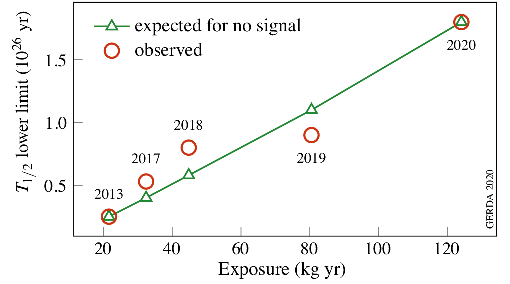
\includegraphics{figs/0vbb/gerda_sensitivity.pdf}
	\caption{Historical limits on the \novbb{} half life, \Thalf{} (red), and expected median sensitivity assuming no signal, $S^{0\nu}_{1/2}$ (green), of the GERDA experiment~\cite{GERDA2020}.}
	\label{fig:sensitivity_gerda}
\end{figure}

Experiments in the field not only report a limit, but a median sensitivity, $S^{0\nu}_{1/2}$. To do this, a Monte Carlo simulation of an ensemble of identical experiments is conducted. From this ensemble, the median $UL_{90\%}(B)$,  $\langle UL_{90\%}(B) \rangle$, is extracted. Replacing $UL_{90\%}(B)$ with $\langle UL_{90\%}(B) \rangle$ in Eq. \ref{eq:Thalflim} yields the median sensitivity. As seen in Fig.~\ref{fig:sensitivity_gerda}, the limit, $T^{0\nu}_{1/2}$ -- subject to the statistical variation of counts that appear in the ROI -- fluctuates over the lifetime of the experiment, while $S^{0\nu}_{1/2}$ monotonically increases with the exposure in background free regime of the GERDA experiment.

The median sensitivity varies with the energy resolution and the background rate as shown in Fig.~\ref{fig:sensitivity_heat}. Taking a slice at $\mu_b = 8 \times 10^{-6}$ c/(keV\,kg\,yr) in this figure and in Fig. \ref{fig:sensitivity_disc}, the effect of increasing the energy resolution can be observed. This is shown in Fig.~\ref{fig:sensitivity_comp}, where it is clear that the discovery level sensitivity is suppressed to greater extent than median sensitivity at poorer resolutions. Thus, the superb energy resolution of Ge detectors presents a clear advantage in the search for \novbb{}, with Ge-based experiments having a particularly high discovery level sensitivity.
\begin{figure}[H]
	\centering
	\subfigure[]{
		\centering
		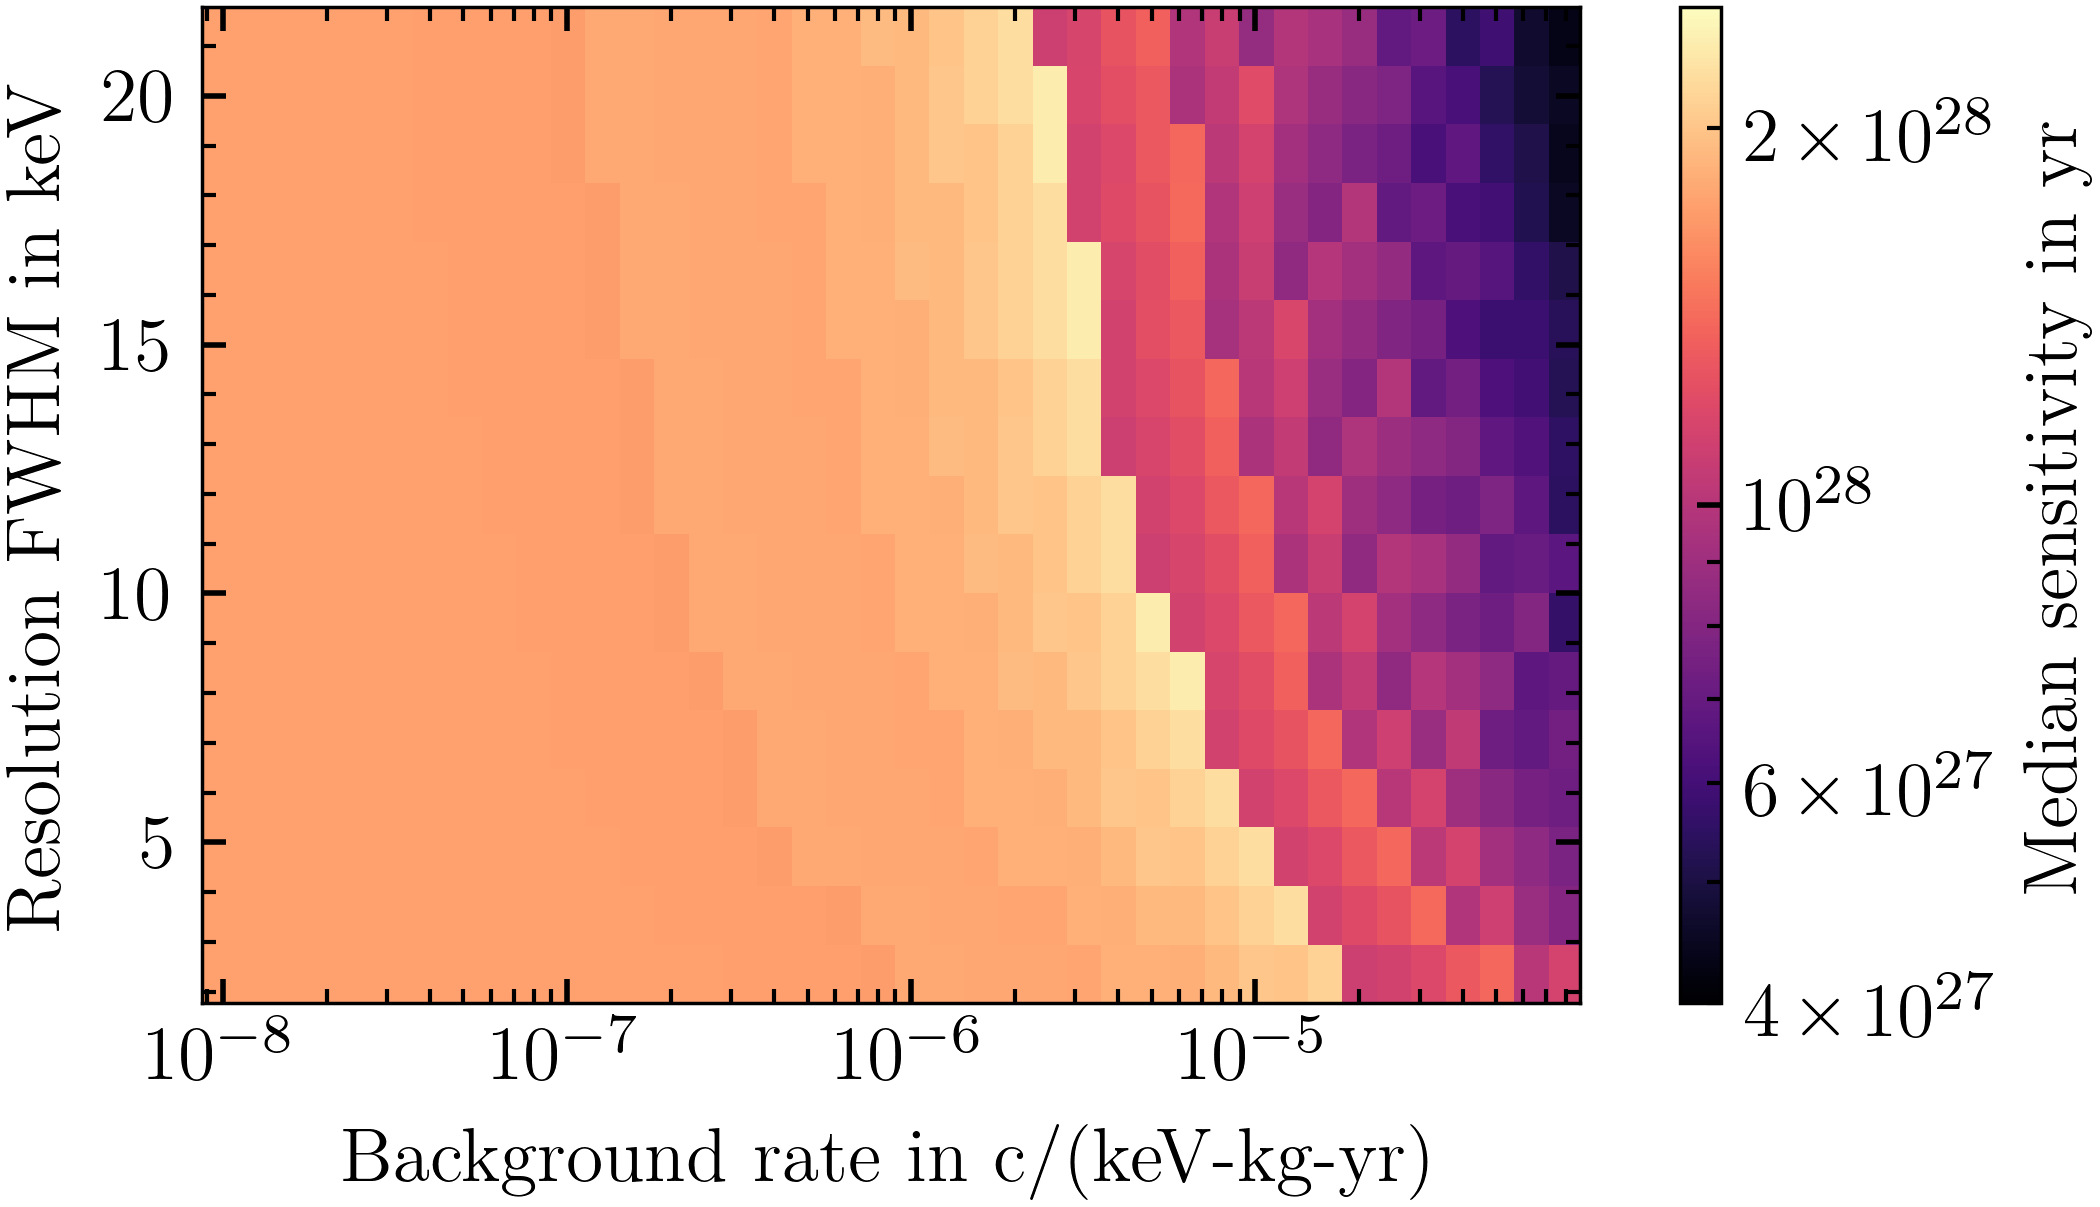
\includegraphics[width=3.7in]{figs/0vbb/median_sensitivity.png}
		\label{fig:sensitivity_heat}
	}
	\subfigure[]{
		\centering
		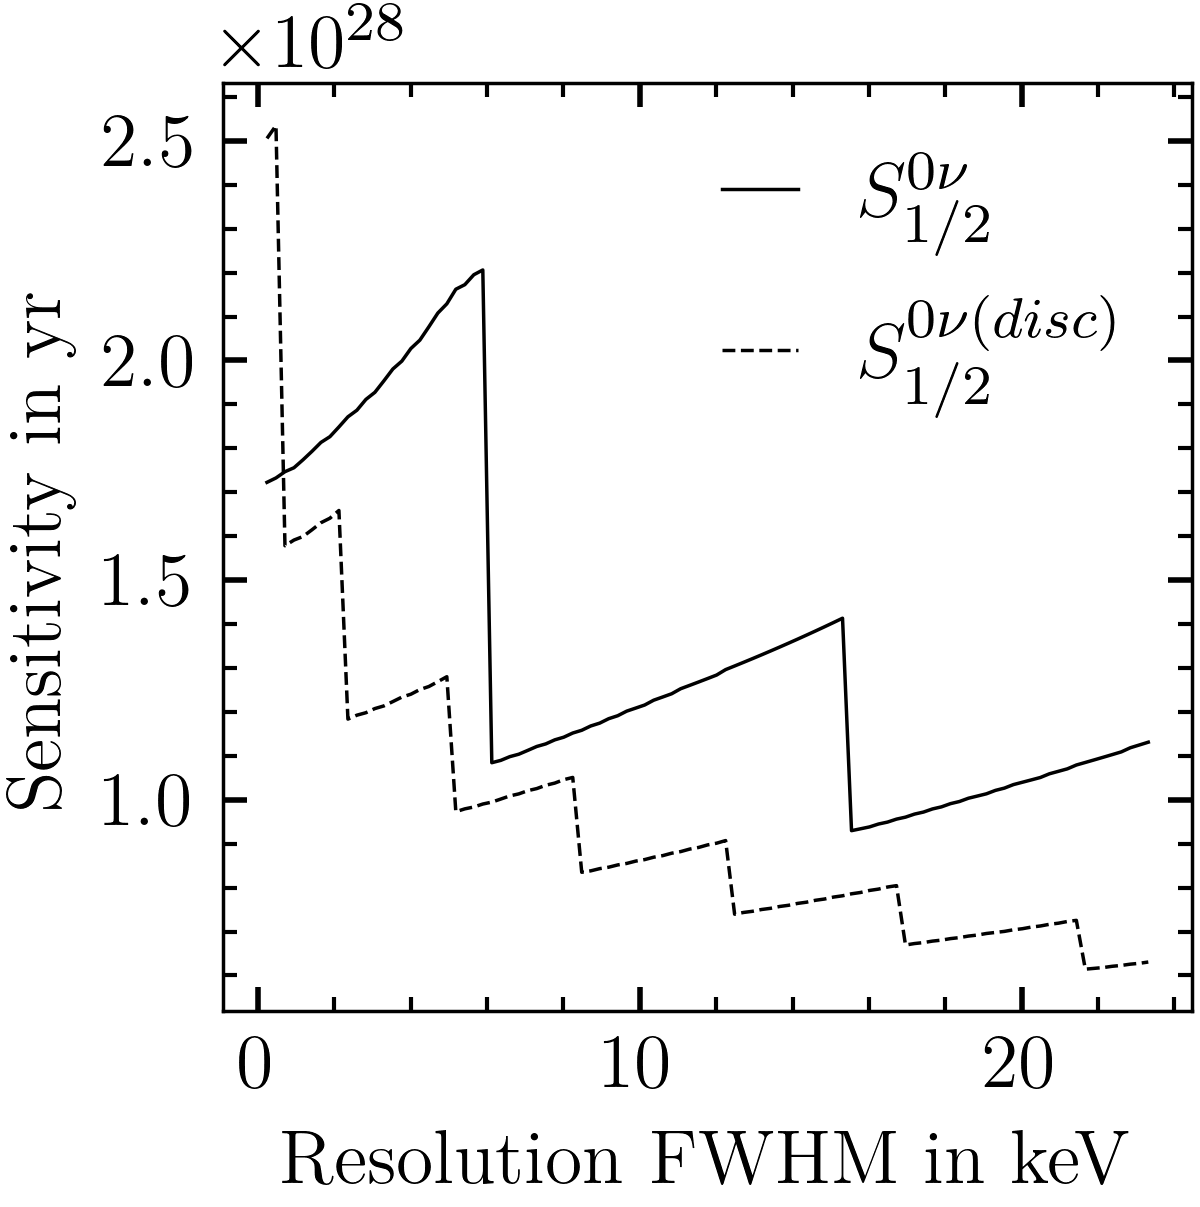
\includegraphics[width=2.1in]{figs/0vbb/discvslim.png}
		\label{fig:sensitivity_comp}
	}
	\caption{(a) Median sensitivity, $S^{0\nu}_{1/2}$, assuming no signal, for a 1 tonne \geEn{} experiment with 10 year live time, as it varies with respect to the background rate and energy resolution of the experiment. Assumes 100\% enrichment, $\epsilon_{tot} = 0.8$, and \twovbb{} contamination. Exactly 1000 identical experiments are simulated in each case. (b) Median sensitivity, assuming no signal (solid black, as calculated from 10,000 identical simulated experiments), and discovery level sensitivity (dashed black) as it varies with energy resolution.} 
	\label{fig:sensitivity}
\end{figure}

\section{Searching for \novbb{} With Germanium Detectors} \label{sec:bg_disc}

In \novbb{}, two electrons carry all the energy available in the decay. Due to the high density of \geEn{}, the range of electrons is limited to 1\,mm. Therefore, a very high percentage of events are fully contained in the bulk, and the energy is deposited within 1\,mm of the decay vertex. Meanwhile, surface events are likely caused by alpha and beta emitters outside the detector. Therefore, large detectors are desirable since they have a lower surface-to-volume ratio. In Ge full event topology cannot be reconstructed, and event selection is fully based on the modeling of pulse-shapes in the detector. However, the inherent single-site topology of \novbb{} events in dense materials allows for a powerful discrimination of backgrounds.

The 0.5 -- 1 mm thick n$^+$ dead region is too thick for alpha particles to transverse and deposit energy in the ROI. The n$^+$ contact extends over the most of the surface of PPCs, BEGes and ICPCs. However, the small fraction not covered provides an entry window for alpha particles. In {\MJMit} style PPCs in particular, a large fraction of the bottom of the detector is covered by a passivated region, which isolates the p$^+$ and n$^+$ contacts. Events occurring on this surface are characterized by incomplete charge collection due to slow charge drift and trapping on the surface. Therefore, alpha events, which have known energy peaks above 5 MeV, can fall in the much lower ROI of \novbb{}.

Charge trapping along the drift path is a potential issue for all events. Events in the bulk of the detector, such as those triggered by gamma particles are subject to this effect. This can be seen in the low energy tails of known gamma peaks. A bulk-charge trapping correction is applied for such events which mitigates the low energy tailing. On the other hand, charge trapping on detector surfaces is not as well understood and a correction cannot be applied. Nevertheless, these events can still be identified and discarded. By conducting scans with alpha sources on the passivated region of PPC detectors, the delayed charge recovery (DCR) effect was observed. A fast pulse with incomplete charge will form in the detector, thus resulting in a degraded energy reading. As the event progresses, charge carriers at the detector surface are released over time, resulting in a positive slope of the charge signal tail. In the {\DEMit}, the DCR parameter was developed to systematically identify and remove these events, resulting in a drastic reduction of surface events falling in the \novbb{} ROI~\cite{dcr}. A careful handling of the detectors and supporting structural materials further aids in the reduction of surface backgrounds. For example, Ge detectors are kept in vacuum or in nitrogen-flushed environments to avoid deposition of the alpha-emitting $^{222}$Rn found in air.
\begin{figure}[htb]
	\centering
	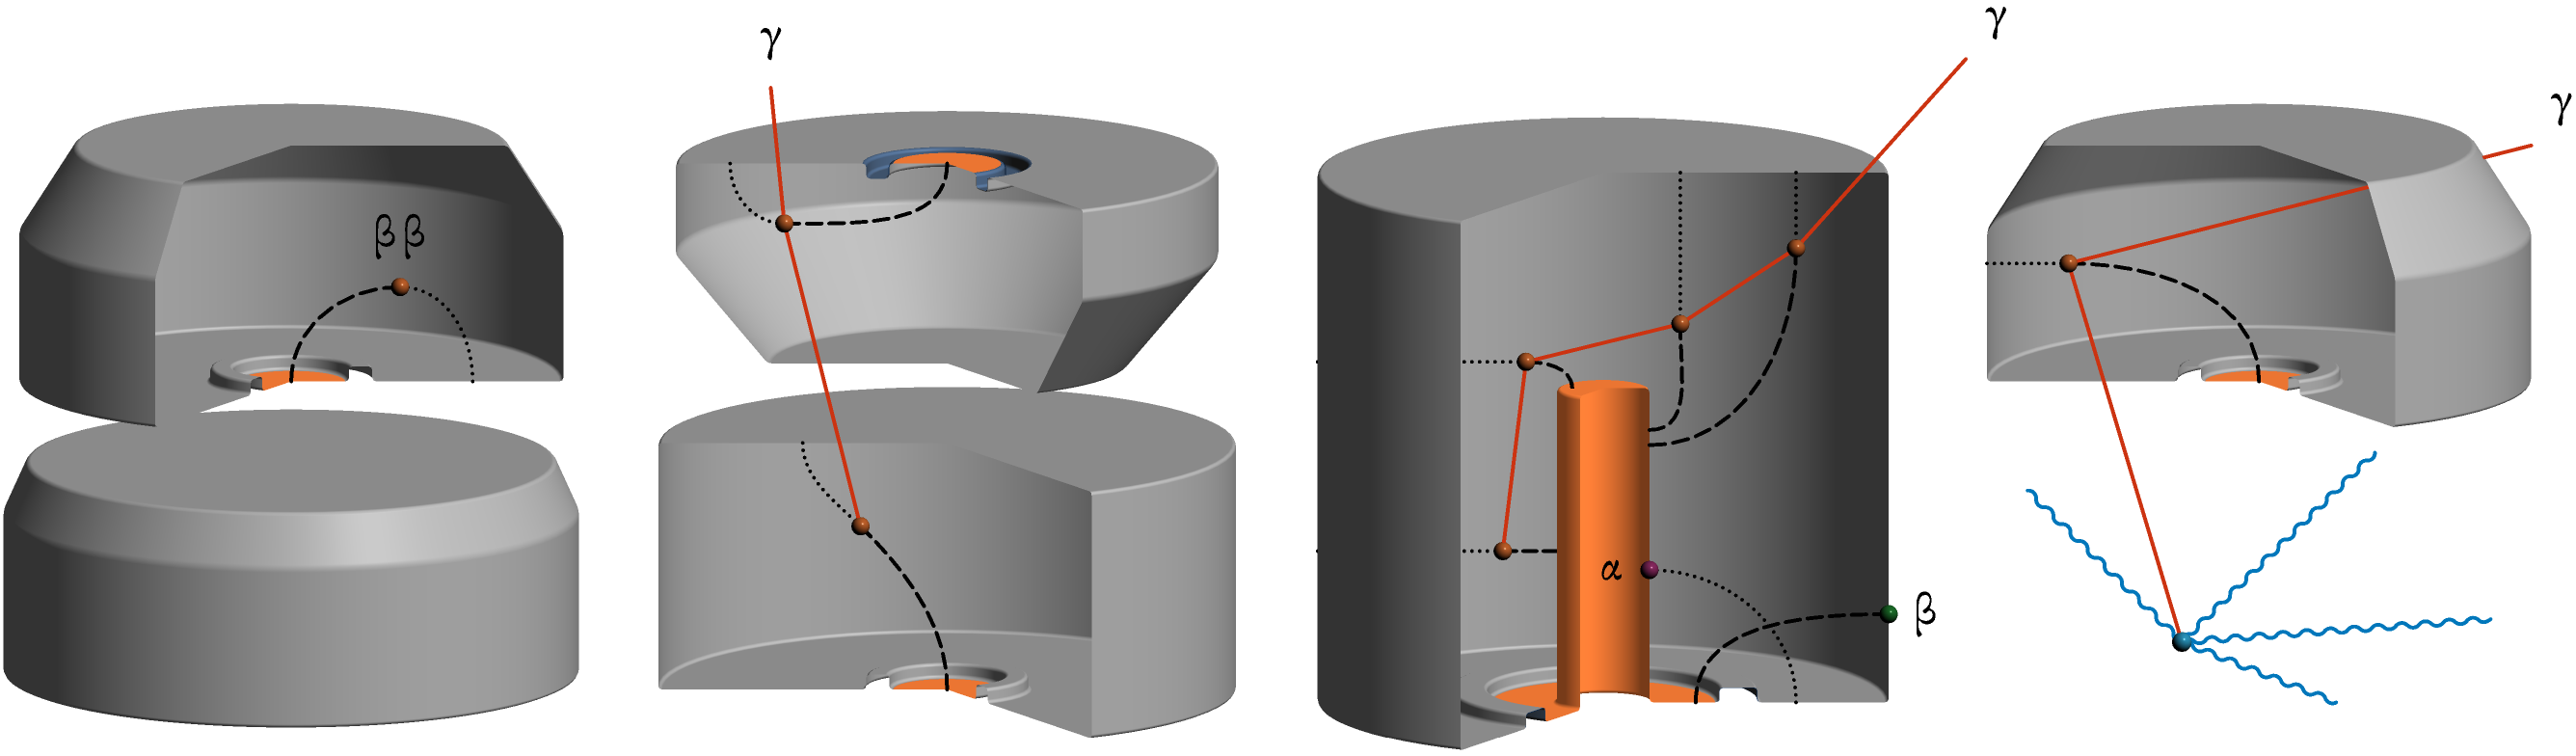
\includegraphics[width = \linewidth]{figs/0vbb/bkg_events.png}
	\caption{Background mitigation strategies. From left to right: illustration of the acceptance of $\beta\beta$ events, rejection of coincident events between two neighboring detectors, rejection of multi-site and surface events and rejection of coincident events between a detector and LAr. p$^+$ contacts are shown in orange~\cite{legend_website_detectors}.} 
	\label{fig:bkg_disc}
\end{figure}

Other surface events include energy depositions in the transition region between the n$^+$ contact and the bulk of the detector. The so-called late charge (LQ) parameter is determined by the ``integral of uncollected charge after a waveform has reached 80\% of its maximum value''~\cite{mjd_final}. Charge carriers produced in this region slowly diffuse to the bulk of the detector, resulting in increased pulse rise times and characteristically high LQ. Finally, p$^+$ contact events are characterized by abnormally fast pulse rise times and thus exhibit a large current amplitude, $A$, with respect to the event energy $E$. By dividing $A$ by $E$ a discriminator against these, and other, events is created -- the $A/E$ parameter. p$^+$ contact events can be removed by a high-$A/E$ cut. 

Events in the bulk of the detector can also originate from backgrounds. Gamma particles can fully transverse the detector; therefore, Compton scatters originating from full energy peaks above \Qbb{} can produce signals in the ROI. Of particular concern are the primordial isotopes $^{232}$Th and $^{238}$U, whose decay chains contain $^{208}$Tl and $^{214}$Bi respectively. The corresponding prominent 2615\,keV and 2204\,keV gamma peaks are well above \Qbb{} and can be observed in the spectra of \geEn{}-based experiments (Fig.~\ref{fig:mjd_spectrum} and Fig.~\ref{fig:gerda_spectrum}). $^{232}$Th and $^{238}$U can be found in virtually all earth-based materials. The fist line of defense against such contaminants is not introducing them in the first place. For this reason, the materials chosen to build \novbb{} experiments, particularly materials close to the detector(s), undergo extensive radiopurity screening and selection.

If a gamma particle scatters and deposits energy in more than one vertex in the detector -- a so-called multi-site event -- the resulting pulses will exhibit an extended multistep current amplitude. The amplitude will be degraded with respect to a single-site event of the same energy. Therefore, multi-site events can be removed by a low $A/E$ cut. The $A/E$, LQ and DCR discriminators are examples of pulse-shape discrimination (PSD) techniques.
\begin{figure}[htb]
	\centering
	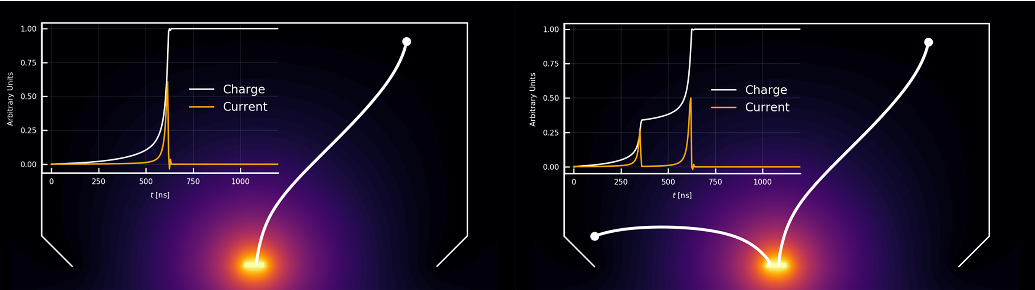
\includegraphics[width=6in]{figs/0vbb/sse_mse.pdf}
	\label{fig:mse}
	\caption{A multi-site event (right) presents an extended multistep current amplitude with respect to that of a single-site event (left) of the same total energy and thus rejected. These events are simulated in a PPC detector. The energy deposition locations and drift paths are shown in white and overlaid on the PPC's weighting potential. The outline of the detector is also shown in white.} 
\end{figure}

If gamma particles scatter in a detector and escape, a different approach is needed. Such events can be vetoed via anti-coincidence cuts if they deposit energy in any other active material in the experiment, which could be another Ge detector. In this regard, surrounding the detectors by active material is beneficial. For example, operating the detectors in liquid argon (LAr) provides an active medium which scintillates when struck by Compton scattered gammas. The light can be read out by instrumenting the LAr. However, the LAr itself, which is in contact with the germanium, is a source of additional backgrounds. Therefore, this approach comes at a higher risk when compared to the traditional operation of detectors in vacuum. The {\MJDEMit} and GERDA experiments highlight the difference between these approaches.

\section{Present and Future Experiments} \label{sec:experiments}

The {\MJMit} collaboration searched for \novbb{} in \geEn{} using enriched, high-purity Ge (HPGe) detectors. The {\MJDEMit} consisted of an array of HPGe detectors located in the Sanford Underground Research Facility (SURF) in Lead, South Dakota~\cite{mjd}. The ultra-low background and record energy resolution achieved by the {\DEMit} enabled a sensitive \novbb{} search, as well as additional searches for new exotic physics~\cite{mjd_axions, mjd_trinucleon,mjd_waveform}.
\begin{figure}[htb]
	\centering
	\subfigure[{\MJDEMit}]{
		\centering
		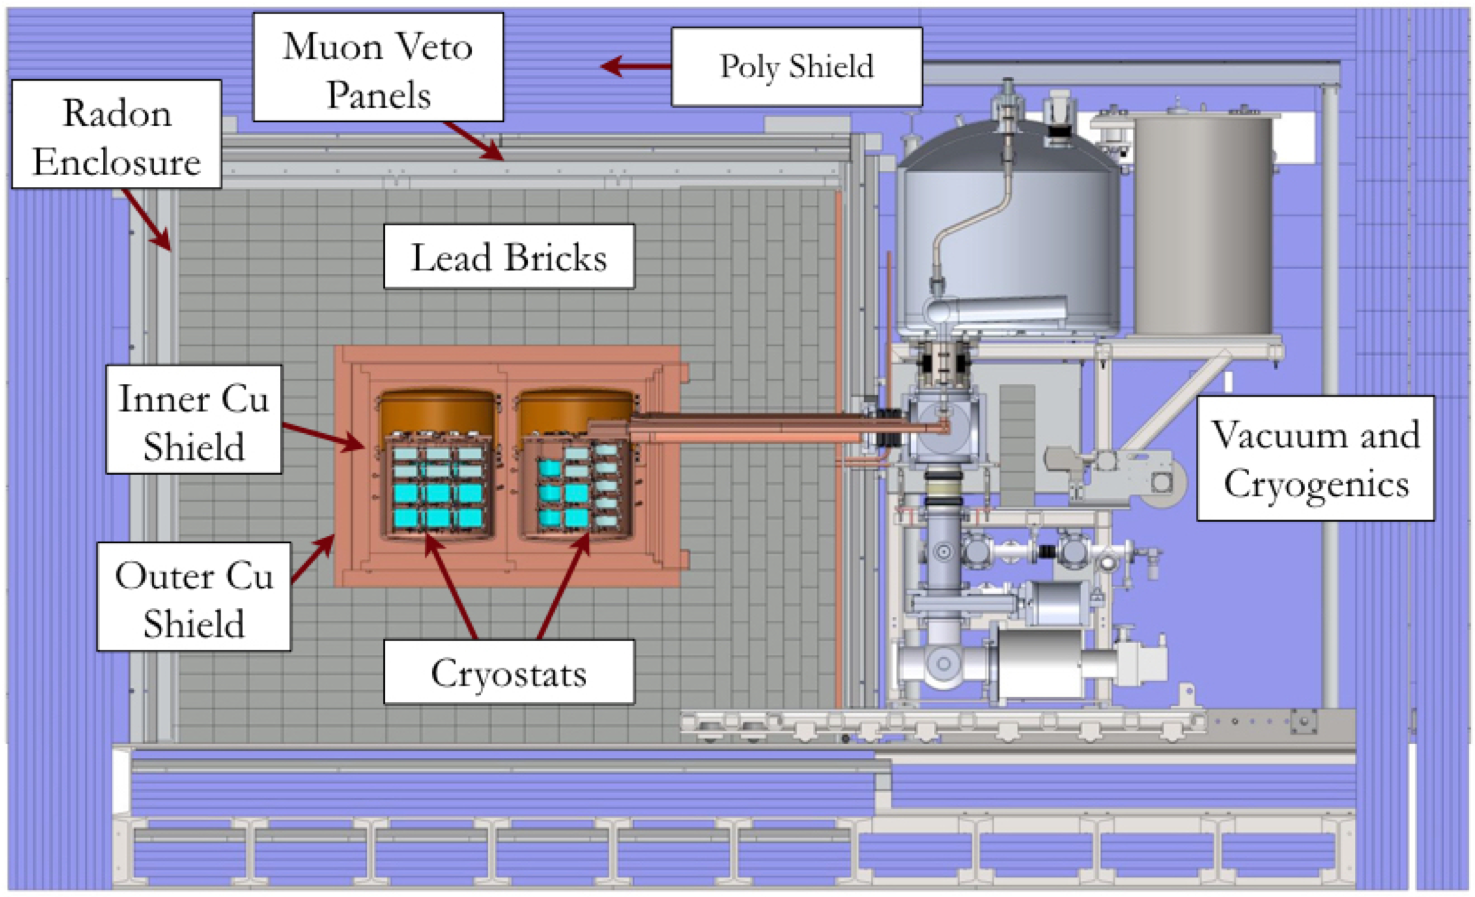
\includegraphics[height = 0.3\linewidth]{figs/0vbb/mjd}
		\label{fig:mjd}
	}
	\subfigure[GERDA]{
		\centering
		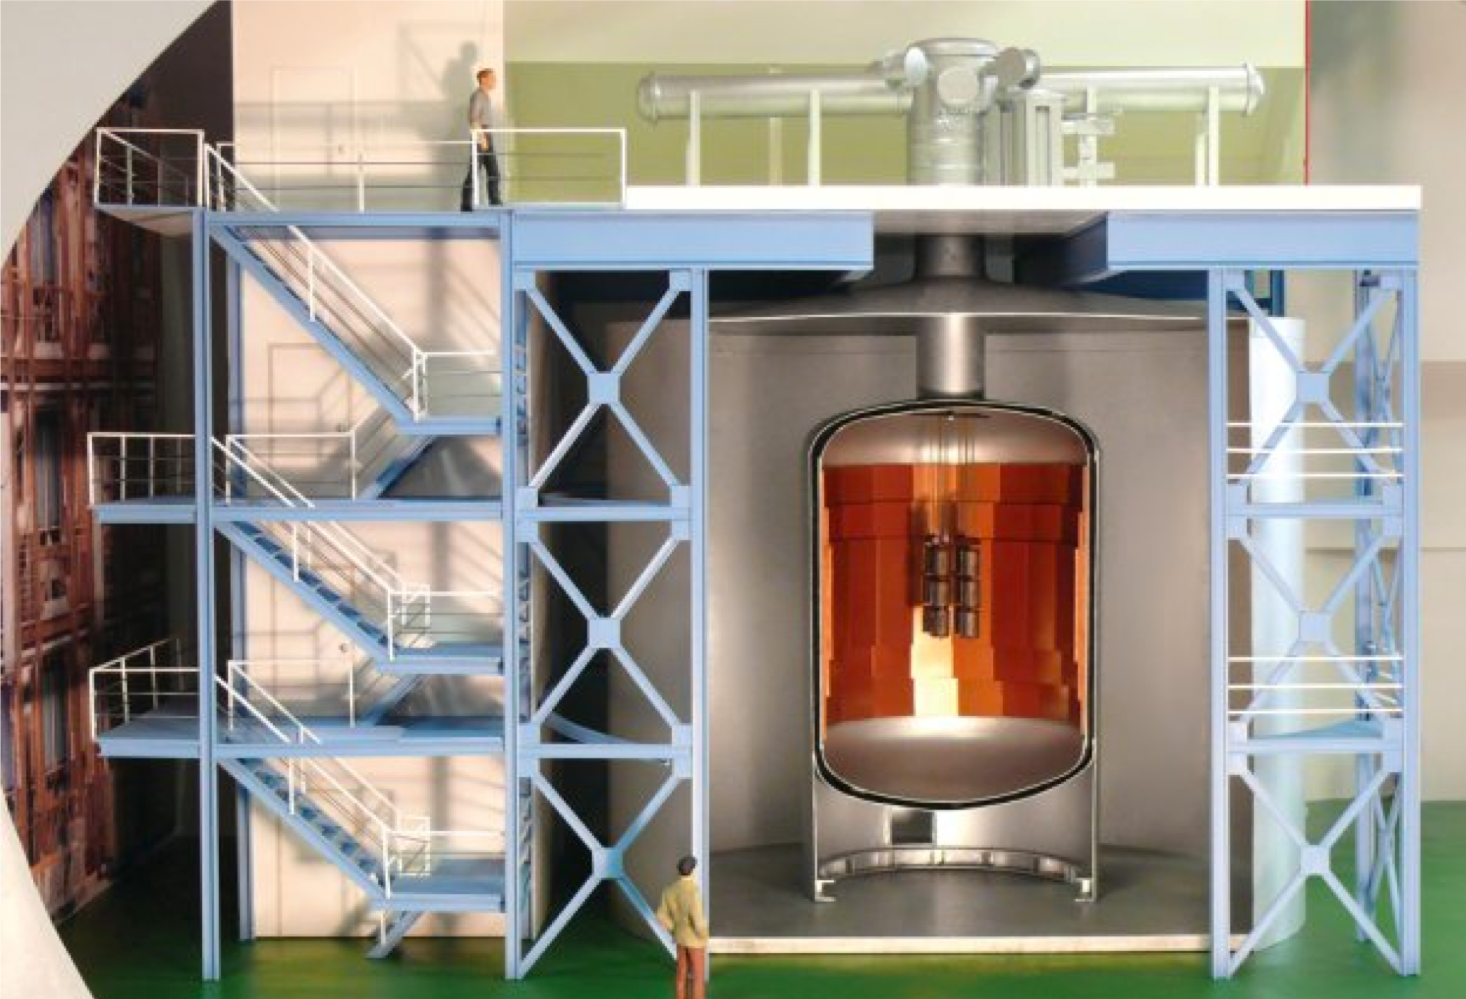
\includegraphics[height=0.3\linewidth]{figs/0vbb/gerda}
		\label{fig:gerda}
	}
	\caption{ The {\MJDEMit} (a) and GERDA (b) experiments.} 
	\label{fig:experiments}
\end{figure}

The {\MJDEMit} consisted of two modules with a total of 40.4\,kg of HPGe detectors (27.2 kg enriched to 88\% in \geEn{}) operated in vacuum. Initially, all enriched detectors were of PPC geometry; however, in the final stage of data taking five PPCs were replaced by four ICPC detectors. Both vacuum cryostats and all structural components of the detector arrays were machined from ultra-low-background underground electroformed copper (UGEFCu)~\cite{ugefcu} and low-background plastics. Low-radioactivity Parylene was used to coat UGEFCu threads to prevent galling and for the cryostat seal~\cite{mjd_og}. A layered shield enclosed both modules. The innermost layer consisted of 5\,cm of UGEFCu. Five cm of commercial oxygen-free high conductivity copper (OFHCu) and 45\,cm of high-purity lead followed. The shield and module volume were constantly purged with low-radon liquid nitrogen boil-off gas. The aluminum enclosure that isolated this Rn-excluded region, was covered with a plastic active muon veto which provided near-$4\pi$ coverage~\cite{muonveto}. The near-detector readout system, which was integrally designed for the {\DEMit}, included low-mass front end (LMFE) electronics~\cite{lmfe} and low-mass cables and connectors~\cite{cables}. Cables were guided out of each module following a UGEFCu cross-arm which penetrated the layered shield. The cross-arm connected the cryostat with vacuum and cryogenic hardware. Control and readout electronics were just outside the Rn-excluded region. The entire assembly was surrounded by 5\,cm of borated and 25\,cm of pure polyethylene to shield against neutrons.
\begin{figure}[tbh]
    \centering
    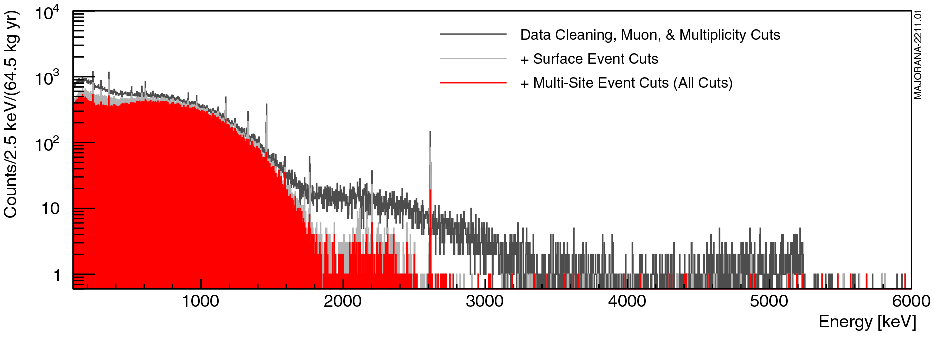
\includegraphics[width=6in]{figs/0vbb/mjd_spectrum.pdf}
    \caption{``The measured energy spectrum above 100\,keV for the [{\MJDEMit}'s] full enriched exposure after applying multiplicity and data cleaning cuts (dark gray), DCR, high-$AvsE$ and LQ cuts (light gray), and the low-$AvsE$ cut (red)''~\cite{mjd_final}}
    \label{fig:mjd_spectrum}
\end{figure}

The {\MJDEMit} applied the discussed DCR, high-LQ and high-and-low-$AvsE$ (similar to $A/E$) cuts to reject backgrounds. After cuts, the {\DEMit} set a lower limit of $T^{0\nu}_{1/2} > 8.3\times10^{25}$ years and reached a sensitivity of $S^{0\nu}_{1/2} = 8.1\times10^{25}$ years, with an exposure of 64.5\,kg\,yr. The corresponding background rate is of $6.6\times10^{-3}$ c/(keV\,kg\,yr)~\cite{mjd_final}. Although the measured background is almost 6 times higher than the assay-based model for the {\DEMit} predicts~\cite{assaypaper}, ongoing background modeling efforts point towards an unaccounted $^{232}$Th excess consistent with a source far away from the detectors. Therefore, critical components near the detectors such as UGEFCu parts and LMFE electronics are safe to use in future experiments. The energy resolution achieved by the {\DEMit} -- 2.52 keV FWHM at \Qbb{} -- is the best of any \novbb{} experiment. The lower limit on the half-life was used to calculate an upper limit on the effective Majorana mass using Eq.~\ref{eq:Thalfexp} and values from literature. Using ``a range of $M_{0\nu}$ values of 2.66-6.34, phase space factors ($G_{0\nu}$) of $2.36\times10^{-15}$ or $2.37\times10^{-15}$, and an effective axial weak coupling of $g^\text{eff}_A=1.27$ for free nucleons''~\cite{mjd_final} gives an upper limit on \mbb{} in the range of 113-269\,meV. In fulfillment of its experimental goals, the {\MJMit} collaboration has demonstrated backgrounds low enough to warrant the construction of a tonne-scale experiment. 
\begin{figure}[tbh]
    \centering
    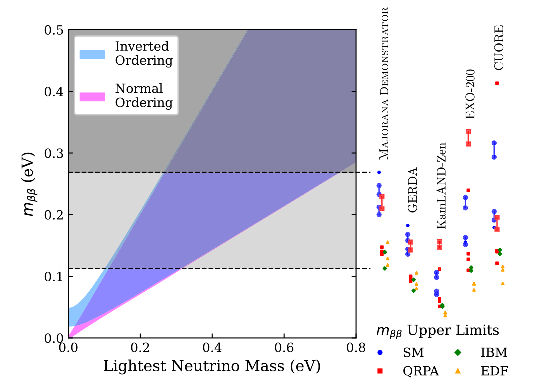
\includegraphics[width=5in]{figs/0vbb/gerda_mjd_limits.pdf}
    \caption{The limit placed on $\langle m_{\beta\beta} \rangle$ by the {\MJDEMit} is shown as a light gray central band in the $\langle m_{\beta\beta} \rangle$ parameter space. A breakdown of this range into the individual upper limits derived from the relevant nuclear matrix elements found in literature is shown on the right. The broken down limits achieved by GERDA (\geEn{}), KamLAND-Zen ($^{136}$Xe), EXO-200 ($^{136}$Xe) and CUORE ($^{130}$Te) are also included~\cite{mjd_final}.}
    \label{fig:gerda_mjd_limits}
\end{figure}

The Germanium Detector Array (GERDA) collaboration operated an array of \geEn{}-enriched HPGe detectors at Laboratori Nazionali del Gran Sasso (LNGS) in Italy. The detectors used were also of p-type point-contact technology: BEGes and ICPCs. GERDA took a novel approach to background suppression based on a LAr active veto~\cite{lar_veto}.  This is in direct contrast to the tried and true detector-in-vacuum approach of the {\MJDEMit} and others before it, such as the Heidelberg-Moscow and IGEX experiments~\cite{h-m, igex}. The GERDA detector strings were suspended in LAr and surrounded by a shroud of silicon-photomultiplier-coupled wavelength shifting fibers. Background suppression was achieved by anti-coincidence cuts between events read out by Ge detectors and scintillation light collected by the fiber shroud. In addition, also in contrast with the {\DEMit}, GERDA opted for a water Cherenkov muon veto, which encapsulated the LAr cryostat. The GERDA water tank was lined with photomultipliers that read out the Cherenkov light produced when a muon interacted in the water. 

GERDA used a single parameter, $A/E$, to perform all background cuts. In BEGe and ICPC detectors, the passivated surface, is much smaller than in the {\MJMit} PPCs. Given its proximity to the p$^+$ contact, events occurring on this surface can be cut with a high-$A/E$ cut. Additionally, the standard low-$A/E$ cut is used to reject multi-site events. GERDA achieved a lower limit of $T^{0\nu}_{1/2} > 1.8\times10^{26}$ years with an exposure of 103.7\,kg\,yr. The corresponding upper limit on the effective Majorana mass is $\langle m_{\beta\beta} \rangle < 79-180\text{\,meV}$. Fig.~\ref{fig:gerda_mjd_limits} summarizes the best limits set on $\langle m_{\beta\beta} \rangle$ by the {\MJDEMit}, GERDA and other experiments searching for \novbb{} in different isotopes. GERDA's background rate is $5.2\times10^{-4}$ c/(keV\,kg\,yr) -- the lowest of any \novbb{} experiment~\cite{GERDA2020}. This equates to under 1 count in the ROI given the GERDA exposure -- a quasi-background-free level -- and has set the standard for the next generation of experiments.

\begin{figure}[tbh]
    \centering
    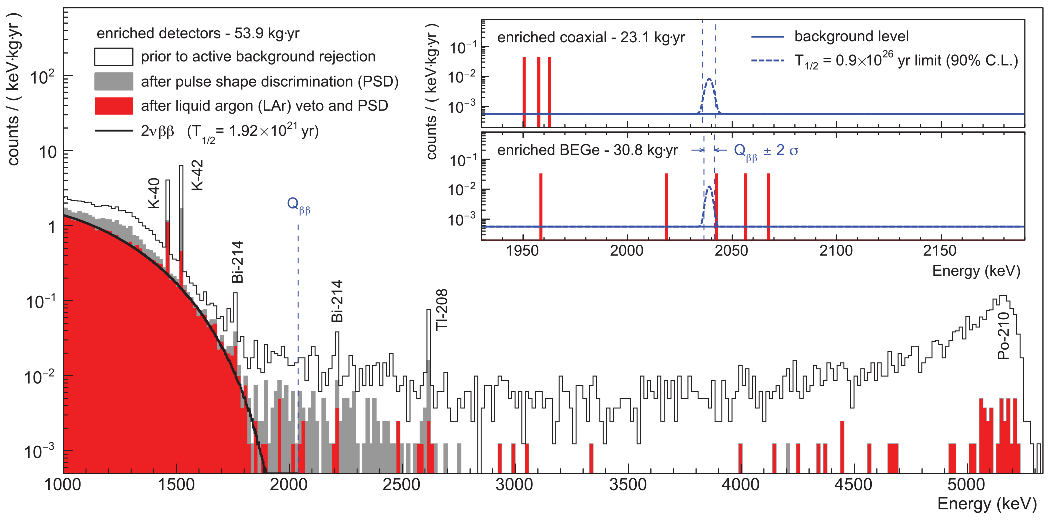
\includegraphics[width=6in]{figs/0vbb/geda_spectrum_breakdown.pdf}
    \caption{``GERDA Phase II energy spectra (53.9\,kg\,year). Enriched coaxial and BEGe data are displayed in a combined spectrum after indicated cuts. Main contributions to the spectra are labeled. The insets display the analysis window for coaxial and BEGe detectors separately, including the background rates (solid blue lines). No event reconstructs within $Q_{\beta\beta} \pm 2\sigma$. The dashed blue curves depict the 90\% C.L. limit for a \novbb{} signal of $T^{0\nu}_{1/2} = 0.9\times10^{26}$ years derived from the likelihood analysis of all GERDA datasets.''~\cite{gerda}}
    \label{fig:gerda_spectrum}
\end{figure}  

Fig.~\ref{fig:mjd_spectrum} and Fig.\ref{fig:gerda_spectrum} show the final spectra of the {\DEMit} and a GERDA spectra with similar exposure respectively. The GERDA spectrum demonstrates the self-vetoing power of the instrumented LAr. The LAr introduces $^{42}$K, a daughter of the long-lived $^{42}$Ar found in atmospheric Ar. $^{42}$K undergoes beta decay, and the progeny de-excites resulting in a 1525\,keV gamma line. These gammas and associated Compton scatters are seen in the Ge spectra. If the associated beta particles deposit energy in the LAr, such events can be vetoed by applying the anti-coincidence cut. Note that a prominent $^{42}$K peak is not present in the {\DEMit}'s spectra. The LAr is also particularly effective at eliminating events in the Compton continua of the $^{208}$Tl and $^{214}$Bi peaks, resulting in a strong background suppression in the \novbb{} ROI. This region is dominated by passivated surface events in the spectra of the {\DEMit}. After all cuts, a higher background still remains, which is suspected to originate from the Compton continuum of $^{208}$Tl, indicating the presence of the aforementioned $^{232}$Th contaminant. By comparing the full spectrum before cuts to the prominence of the \twovbb{} spectrum in the GERDA and {\MJDEMit} spectra the effect of running in LAr vs. in vacuum can be observed. A lower background is observed in the {\DEMit} in the (1000-1500)\,keV and > 3000\,keV regions due to the $^{42}$K gammas and $^{42}$K betas and other alpha emitters in GERDA respectively. The {\MJDEMit}'s focus on ultra-low background construction materials and careful handling and tracking of parts is responsible for its low background before cuts. 

It is clear that the experimental strategies of GERDA and the {\MJDEMit} are complimentary and should be combined. Drawing from both experiments, a new collaboration was born. GERDA achieved its experimental design goal of 100\,kg\,yr of exposure, and its infrastructure now houses the first phase of the next generation \novbb{} experiment in \geEn{}: The Large Enriched Germanium Experiment for Neutrinoless Double-Beta Decay (LEGEND-200).